\documentclass[12pt,twoside]{report}
\usepackage[utf8]{inputenc}
\usepackage[english]{babel}
\usepackage{csquotes}
\usepackage{amssymb}
\usepackage{amsmath}
\usepackage{mathrsfs}
\usepackage{tikz}
\usepackage{forest}
\usepackage{pgfplots}
\pgfplotsset{compat=1.7}
\usepackage[a4paper,width=150mm,top=25mm,bottom=25mm]{geometry}
%\usepackage[a4paper,left=3cm,right=2cm,top=2.5cm,bottom=2.5cm]{geometry}
\usepackage{marginnote}
\usepackage[makeroom]{cancel}
\usepackage[ruled,vlined,linesnumbered]{algorithm2e}
\usepackage{algorithmic}

\usepackage[
    backend=biber,
    style=alphabetic,
    sorting=ynt
]{biblatex}




\addbibresource{mybib.bib} %Imports local bibliography file



\title{Master Thesis}
\author{Alberto Tiraboschi}
%\date{ }

\begin{document}

\numberwithin{equation}{section}

\maketitle
\clearpage
\thispagestyle{empty}
\tableofcontents
\thispagestyle{empty}
\clearpage

\setcounter{page}{1}

\chapter{Abstract, possibili applicazioni, descrizione (1 pg)}
Scopo della tesi fare un po di ordine nello stato attuale degli algoritmi di ricerca tramite rssi. qui faccio un revisiting dei piu noti algoritmi, cercando di mediare fra la teoria e l'applicazione, adattando i modelli proposti in una forma che si presta meglio all'implementazione algoritmica.
\clearpage

\chapter{Modello matematico della propagazione del segnale (2 pag)}
\section{Path loss model}
The log-normal propagation model, see \cite{MUNOZ200923}, is
\begin{equation}
\upsilon(d) = A-10\alpha\log_{10}\bigg(\frac{d}{d_0}\bigg) + \xi, \quad d>d_0
\end{equation}
where $\xi$ is a zero-mean gaussian variable that represents the noise, $\alpha$ is the path loss index, which can vary between $2$ (open field) and $4$ (environment fitted with obstacles) and $A$ is the $RSSI$ read at $d_0$. Commonly $d_0$ is taken as $1$ meter, so that we can simplify the ?? as
\begin{equation}
\upsilon(d) = A-10\alpha\log_{10}(d) + \xi   
\end{equation}
In some algorithms that don't not require a high precision the noise is not taken into account. Instead for some other algorithms it is a good idea to rewrite the model as follows, by letting $\beta=10\alpha/\ln(10)$:
\begin{equation}
\upsilon(d) = A-\beta\ln(d) + \xi
\end{equation} where $\ln(\bullet)$ is the natural logarithm, and then deriving a slightly different model
\begin{equation}
\nu(d) = \upsilon(d)-A= -\beta\ln(d) + \xi
\end{equation}
\clearpage


\chapter{Disturbances of RSSI}
The RSSI noise has a great influence over the measurements, thereby complicating the attempt to get precise location. To give some numbers, the available range of signal intensity that a common WiFi device can measure varies in the interval $-30\div-90$ dbm and the value obtained can generally deviate from the exact value at most $6$ dbm which is as much as $10\%$ over the range of measurement.
Due to its significant influence, it has been investigated many times in order to discover some patterns, but up to now no answer has been found. For example \cite{4608603} showed that there are no significant patterns over the time domain neither in the frequency domain. Instead the causes of the noise are well known and are the same that affects the propagation of any electromagnetic wave.
We can summarize two main issues that cause RSSI instability: 
\section{Multipath Fading, NLOS propagation} 
As outlined in \cite{onl11}, multipath fading occurs when there are multiple ways for the signal to reach the receiving device. This causes the signal waves to reach the receiving end with in two different times, that is, there is a non negligible delay between the two (or more) waves. This means phase shifting, leading to constructive/destructive interference of the signal. This effect is very preeminent in closed environments, when there are many surfaces able to reflect the signal. It is totally randomic \cite{10.5555/559977} therefore it is unpredictable by definition. The good new is that it can be removed by filtering the outliers, with some of the methods presented later.
\section{Shadow Fading}
This effect is the attenuation of the signal caused by heavy and large (w.r.t. the wavelength) obstacles between the receiver and the sender that adsorb (or may even block) the waves. This is classically related to NLOS (Non Line Of Sight) environments that is, when the signal is not receiver cannot "see" the sender. This effect is taken into account in the model as the path loss index $\alpha$. This is quite a problem when there are many obstacles obstructing the way, therefore the correct path loss index can only be estimated with some algorithms, one of them is presented later, and not analitically computed. It showed spatial correlation \cite{244122,732812}, which is in fact intuitive, all the measurements taken in a certain position, with a certain number of obstacles will be all affected by an almost equal shadow fading, whereas in another locations it will not. The problematic effect of this noise is that is shows a systematic behaviour, in other words, each measurement is affected by an almost equal way, therefore trying to remove it by removing outliers is not an effective way. If the path loss index is taken wrong in the model for some reasons, the estimated position will be altered with some significant errors, that may set negligible the improvement of other source of noise. Even more complicate is when there are persons moving freely between the sender and the receiver. The body of each passing person adsorb the signal, therefore alterating the measure. The estimated position will inevitably bear some non negligible errors.

\chapter{Noise removal}
I will present here some method to remove outliers in a series of data. I will present them from a mathematical point of view before, and then an extract of the algorithm in pseudocode.
\subsection{IQR}
This method, whose name is InterQuartile Range method, is based, as the name suggest, on the quartiles of a dataset. I will present an algorithm that can be used to obtain the quartiles. I will assume some facts:
\begin{itemize}
    \item Arrays index starts from zero
    \item Float numbers are cast to integer with truncation of the decimal part
    \item Datasets
    \begin{itemize}
        \item d1
        \item d2
        \item d3
    \end{itemize}
\end{itemize}

\begin{algorithm}[H]
\SetAlgoLined
\KwResult{Q1, Q2, Q3}
d1.sort(ascending)\;
Q1 = Q2 = Q3 = 0\;
s1 = d1.size()\;
\eIf{s1.is\_even()}{
    Q2 = (d1[s1/2 - 1] + d1[s1/2])/2\;
    d2 = d1[0 : s1/2 - 1]\;
    d3 = d1[s1/2 : s1 - 1]\;
}{
    Q2 = d1[s1/2]\;
    d2 = d1[0 : s1/2 - 1]\;
    d3 = d1[s1/2 + 1 : s1 - 1]\;
}

s2 = d2.size()\;
s3 = d3.size()\;
\eIf{s2.is\_even()}{
    Q1 = (d2[s1/2 - 1] + d2[s1/2])/2\;
}{
    Q1 = d2[s1/2]\;
}
\eIf{s3.is\_even()}{
    Q3 = (d2[s1/2 - 1] + d2[s1/2])/2\;
}{
    Q3 = d2[s1/2]\;
}
 \caption{Quartiles computation}
\end{algorithm}
\noindent \\Going back to the IQR method you have to do the following steps:

\begin{algorithm}[H]
\SetAlgoLined
\KwResult{The filtered dataset}
Q1, Q2, Q3 known from the previous algorithm\;
IQR=Q3-Q1\;
$I=[Q1-1.5\cdot IQR,\quad Q2 + 1.5\cdot IQR]$\;
 \While{$k \in [1:n]$}{
    \If{! $dataset[k]\in I$}{
        dataset.remove(k)\;
        k=k-1\;   
  }
    k=k+1\;
 }
 \caption{Outliers removal with IQR}
\end{algorithm}
\noindent \\Here it is given a numeric example. Suppose you have the following dataset $$\{-1.9, 0.3, 3.7, 4.1, 6, 6.1, 7.2, 9, 19\}$$ already sorted, where the first seven nuberers are extracted from $-2+X$, where $X$ follows the uniform distribution in $[0,10]$. The latest two values are possible outliers. Since the size of the dataset is odd, $Q2$ can be found at the fifth position and is $6$. We have then the first half and the second half. Since the first half has an even number of data points, the median of the first half ($Q1$) will be $(0.3+3.7)/2=2$, the same reasoning applies to $Q3$ for the second half, which is equal to $8.1$. Therefore the IQR will be $8.1-2=6.1$ the interval $I$ will be
$$I=[2-1.5\cdot6.1,8.1+1.5\cdot6.1]=[-7.15,17.25]$$
As you can see, the number $19$ will be treated as an outlier anf thus be removed. You can also choose how wide the interval you want it to be, for example if you wanted to be more strict you could choose $1$ instead of $1.5$ as a multiplying factor, obtaining the following interval
$$I'=[2-1\cdot6.1,8.1+1\cdot6.1]=[-4.1,14.2]$$

\subsection{Z-score}
The Z-score is another method to find outliers. In few words, the procedure estimates the sample mean and sample standard deviation as follows
\begin{equation}
    \hat{\mu}=\frac{1}{n}\sum_{i=1}^nx_i
\end{equation}
\begin{equation}
    \hat{\sigma}=\sqrt{\frac{1}{n-1}\sum_{i=1}^n(x_i-\hat{\mu})^2}
\end{equation}
Then we compute the z-score $y_i$ of each value $x_i$
\begin{equation}
    y_i=\frac{x_i-\hat{\mu}}{\hat{\sigma}}
\end{equation}
The filtering process now removes every data whose z-score is outside the interval $[-3,3]$. Here an axample, with the same dataset of the previous algorithm
$$\{-1.9, 0.3, 3.7, 4.1, 6, 6.1, 7.2, 9, 19\}$$
The estimated mean is $\hat{\mu}=5.94$ and the sample standard deviation is $\hat{\sigma}=5.32$. Then the corresponding set of z-scores is
$$\{-1.47, -1.06, -0.42, -0.34, 0.01, 0.02, 0.23, 0.57, 2.45\}$$
note the last value, for the previous algorithm it should have been discarded, but according to this one it is still kept. Clearly you can choose a narrower interval than $[-3,3]$.

\clearpage

\chapter{Algoritmi per la stima di alcuni parametri}
A must be known, since can be regarded as a factory data.
\section{Estimation of path loss index}
For the anchor node $i$, the values are obtained according to the following equation
\begin{equation}
  \upsilon_i=A-10\alpha_i\log_{10}(d_i)+\xi_i
\end{equation}
The above model is basically a constant term added to a zero mean gaussian variable, so from \cite{alma9926534668905776}
\begin{equation}
a+\mathcal{N}(0,\sigma^2)\sim\mathcal{N}(a,\sigma^2)
\end{equation} therefore the ?? is gaussian as follows:
\begin{equation}
    \upsilon_i \sim \mathcal{N}(A-10\alpha_i\log_{10}(d_i),\sigma^2_i)
\end{equation}
which has its probability density function
\begin{equation}
    p(x)=\frac{1}{\sqrt{2\pi\sigma_i^2}}e^{-\frac{1}{2}\frac{(x-\mu)^2}{\sigma^2_i}}
\end{equation}
where
\begin{equation}
    \mu = A-10\alpha_i\log_{10}(d_i)
\end{equation}
Given a sample $1<j<m$ of measurements, all given by the same node, that is, that follow the distribution ?? we can employ the Maximum Likelihood to estimate the path loss index specific of this anchr node. It follows
\begin{equation}
    L_m^i(\alpha_i,\sigma_i^2)=
    \frac{1}{(2\pi\sigma_i^2)^{\frac{m}{2}}}e^{-\frac{1}{2}\sum_{j=1}^m\frac{(\upsilon_j-\mu)^2}{\sigma^2_i}}
\end{equation}
by applying the logarithm to both members
\begin{equation}
    \ell_m^i(\alpha_i,\sigma^2_i)=-\frac{m}{2}\ln(2\pi\sigma^2_i)-\frac{1}{2\sigma^2_i}\sum_{j=1}^m(\upsilon_i-\mu)^2
\end{equation}
Maximizing $\ell_m^i$ w.r.t to $\alpha_i$ is equal to minimize the second term in the above equation, therefore \cite{MUNOZ200923} 
\begin{equation}
\frac{\partial}{\partial \alpha_i} \frac{1}{2\sigma^2_i}\sum_{j=1}^m(\upsilon_i-\mu)^2 =0
\end{equation}
\begin{equation}
\frac{\partial}{\partial \alpha_i} \frac{1}{2\sigma^2_i}\sum_{j=1}^m(\upsilon_i-A+10\alpha_i\log_{10}(d_i))^2 =0
\end{equation}
\begin{equation}
\frac{\partial}{\partial \alpha_i} \frac{1}{2\sigma^2_i}\sum_{j=1}^m(\upsilon_j-A+10\alpha_i\log_{10}(d_i))^2 =0
\end{equation}
\begin{equation}
\frac{1}{2\sigma^2_i}\sum_{j=1}^m2\big(\upsilon_j-A+10\alpha_i\log_{10}(d_i)\big)(10\log_{10}(d_i)) =0
\end{equation}
\begin{equation}
\sum_{j=1}^m\big(\upsilon_j-A+10\alpha_i\log_{10}(d_i)\big) =0
\end{equation}
\begin{equation}
\sum_{j=1}^m\upsilon_j-mA+10m\alpha_i\log_{10}(d_i)=0
\end{equation}
\begin{equation}
    \alpha_i=\frac{mA-\sum_{j=1}^m\upsilon_j}{10m\log_{10}(d_i)}
\end{equation}
The path loss index can also be approximatedby taking the mean of the path loss deduced between the ther nodes..
Important to assume homogeneous distribution of anchor nodes this in conclusions, fai anche qualche immagine.
\section{Estimation of $\sigma^2_i$}
Assume to know...\\
The derivative of ?? w.r.t $\sigma^2_i$ is 
\begin{equation}
    \frac{-m\sigma^2_i+\sum_{j=1}^m(\upsilon_i-\mu)^2}{2\sigma^4_i}=0
\end{equation}
Since $\sigma^2_i>0$ we have
\begin{equation}
    \sigma^2_i=\frac{1}{m}\sum_{j=1}^m(\upsilon_i-\mu)^2
\end{equation}

\clearpage

\chapter{Algoritmi per la stima della posizione(16 pag)}
scrivere vantaggi e svantaggi ognuno, testo algoritmo, dimostrazioni matematiche, commenti e opinioni.
\section{General overview and recurring terms}
We want to locate a device, (with a LOS or NLOS condition ?) by exploiting the relation between the received signal strength and the distance between the source node and the position where the measurement is taken. In real scenarios these samples can be provided mainly in two ways. One typical way is to place various anchor nodes, such that the anchor node $i$, can give samples like $(x_i,y_i,rssi_i)$. The other way, which is lately becoming increasingly used is the employment of a drone, that given some bounds on the area to scan, it collects and outputs the samples, behaving as a "moving" anchor node. We have $n$ anchor nodes with known position, and a $t$-th target node with unknown position.The anchor node $i$ at position $x_i,y_i$ gets the measurement of the $rssi_i$.The data is sent to a central processing device that makes the computations and outputs the estimated position. 

\section{Common Paradigm}
To avoid redundancy, given the fact that each algorithm differences itself from the others only because of the mathematic tools employes, it make sense to focus on it in the description of the algorithms, and to present here the common instructions of those algorithms.
When instead the steps are quite different, there will be a more detailed describtion of all the procedure.

\begin{algorithm}[H]
\SetAlgoLined
Collect the signal strength\;
Eventually process the data\;
\eIf{the method has a closed formula}{
    apply the formula and obtain $\hat{\mathbf{x}}$
}{
    \While{convergence or max iteration reached}{
        update $\hat{\mathbf{x}}$\;
 }
}
return results\;
 \caption{Common steps of localization algorithms}
\end{algorithm}

\section{Classification}
Here follows a quite complete classification of the localization methods considered. Model based means that the algorithms that depart from that node, employs directly the model of log prpagation seen in ??, whereas model free don't use it. Closed formula/iterative methods are quite self explaining. Regarding statistics, the sub-classification is based on the employment of probabilistic parameters, one above all, the variance $\sigma^2_i$ of the noise error $\xi_i$ in the previous ?? that affects the reading. Of course, model free methods, since they do not use the model ??, they do not consider also the variance of the noise, nor any other probabilistic parameters.
\scalebox{0.8}{
\begin{forest}
    for tree={
        grow=0,reversed, % tree direction
        parent anchor=east,child anchor=west, % edge anchors
        edge={line cap=round},outer sep=+1pt, % edge/node connection
        rounded corners,minimum width=15mm,minimum height=8mm, % node shape
        l sep=10mm % level distance
    }
 [Root
 [Model Based
 [Closed Formula
 [W/O Statistics [Trilateration ] [Min-Max ] [Quadratic linearization] [Lines intersection] ]
 [W Statistics [Linear estimation ] [Weighted linear estimation ] ] ]
 [Iterative Methods
 [W/O Statistics [Multilateration ] ]
 [W Statistics [Maximum Likelihood ] ] ] ]
 [Model Free
 [Closed Formula
 [W/O Statistics  [Centroid Algorithm] [DV-Hop Algorithm ] ]]
 [Iterative Methods
 [W/O Statistics  [Fingerprinting
 ] ]]
 ] ]
\end{forest}
}

\clearpage
\section{Trilateration 210}

  \begin{center}
  \textbf{Assume to know:}
  \begin{itemize}
    \centering
    \item $A$
    \item $\alpha$
  \end{itemize}
  \end{center}
Consider the trilateration method from a pure theoretical point of view. For this method it is required to have only 3 anchor nodes. Each of them can output its position $(x_i,y_i)$ along with the rssi read in its position of the unknown node. By exploiting the model of the distance and the rssi read, and assuming no noise or multipath fading at all, one can deduce the distance $d_i$ between the unknown node and current node from the model ?? $n_i$ as follows:  
\begin{equation}
    d_i=\sqrt{(x_u-x_i)^2+(y_u-y_i)^2}=10^{\frac{A-r_{rssi,i}}{10\alpha}}    
\end{equation}
As a consequence we can imagine to draw a circle centered in $(x_i,y_i)$ with radius $d_i$. The unknown node $n_u$ should lay on this circumference. Of course, this is not enough to locate $n_u$. Therefore, we need to get data also from the the other 2 anchor nodes. In this way we can draw 3 circles and obtain a unique point of intersection as shown in \ref{fig:trilOK}. Note that 3 nodes are the minimum number of nodes to have an unambiguous result. In fact, if we were to have only 2 nodes, then there would be 2 possible outcomes (the intersection of two circumferences generally results in 2 points), instead of the required one.
\begin{figure}
    \centering
    \scalebox{1}{
        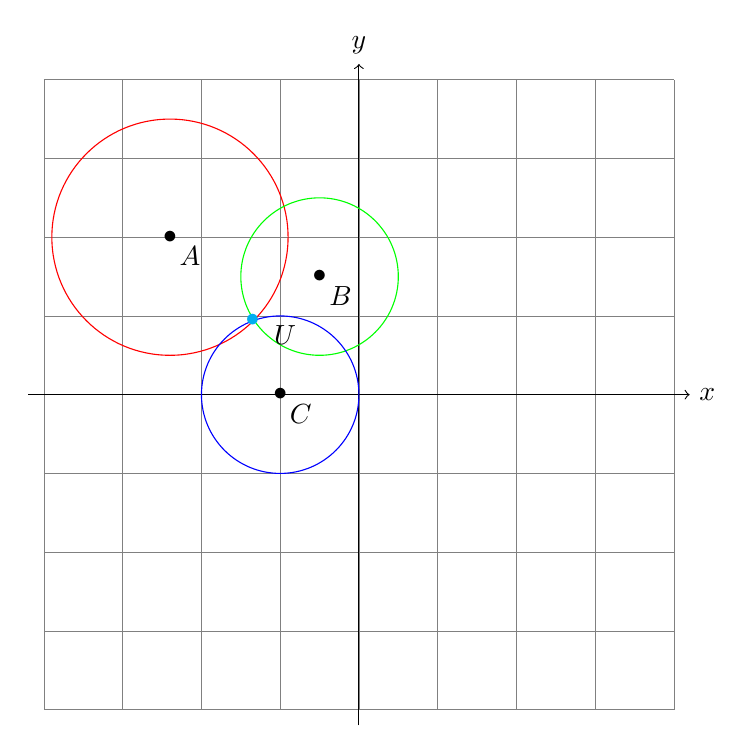
\begin{tikzpicture}
            \draw[very thin,color=gray] (-4,-4) grid (4,4);
            \draw[->] (-4.2,0) -- (4.2,0) node[right] {$x$};
            \draw[->] (0,-4.2) -- (0,4.2) node[above] {$y$};
    
            \draw[color=red] (-2.4,2) circle (1.5);
            \draw (-2.4,2) node {$\bullet$};
            \node[anchor=north west] at (-2.4,2) {$A$};
        
            \draw[color=green] (-0.5,1.5) circle (1);
            \draw (-0.5,1.5) node {$\bullet$};
            \node[anchor=north west] at (-0.5,1.5) {$B$};
        
            \draw[color=blue] (-1,0) circle (1); %2-2sqrt(3)
            \draw (-1,0) node {$\bullet$};
            \node[anchor=north west] at (-1,0) {$C$};
        
            \draw (-1.35,0.95) [cyan] node {$\bullet$};
            \node[anchor=north west] at (-1.2,1) {$U$};   
        \end{tikzpicture}
    }
    %\includegraphics{}
    \caption{}
    \label{fig:trilOK}
\end{figure}
When we step into reality however the disturbances of the signal inevitably lead to wrong estimation of the distance between the current node and the unknown node, causing the circles to intersect in wrong points or to not intersect at all, as in fig. \ref{fig:trilKO}.
\begin{figure}
    \centering
    \scalebox{1}{
        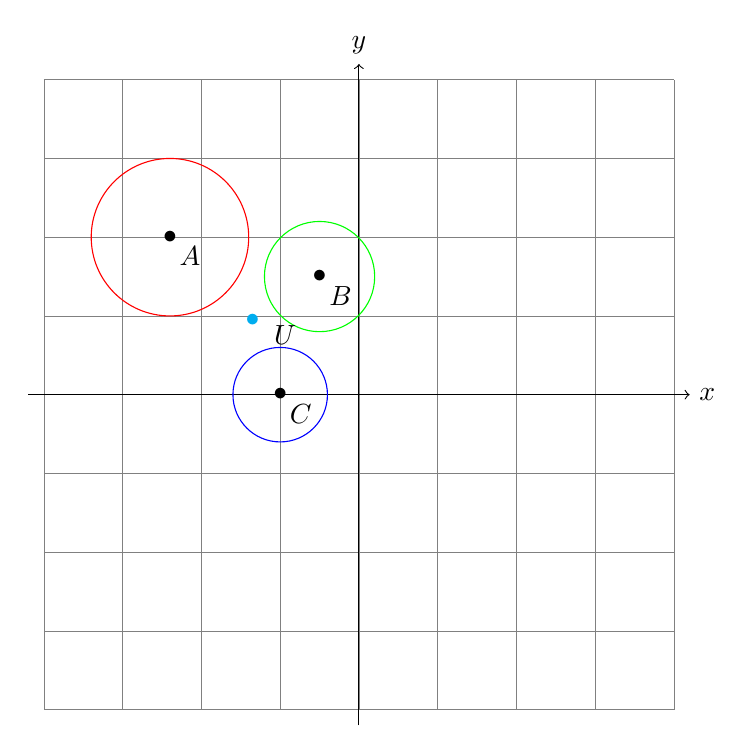
\begin{tikzpicture}
            \draw[very thin,color=gray] (-4,-4) grid (4,4);
            \draw[->] (-4.2,0) -- (4.2,0) node[right] {$x$};
            \draw[->] (0,-4.2) -- (0,4.2) node[above] {$y$};
    
            \draw[color=red] (-2.4,2) circle (1);
            \draw (-2.4,2) node {$\bullet$};
            \node[anchor=north west] at (-2.4,2) {$A$};
        
            \draw[color=green] (-0.5,1.5) circle (0.7);
            \draw (-0.5,1.5) node {$\bullet$};
            \node[anchor=north west] at (-0.5,1.5) {$B$};
        
            \draw[color=blue] (-1,0) circle (0.6); %2-2sqrt(3)
            \draw (-1,0) node {$\bullet$};
            \node[anchor=north west] at (-1,0) {$C$};
            
            \draw (-1.35,0.95) [cyan] node {$\bullet$};
            \node[anchor=north west] at (-1.2,1) {$U$};
        \end{tikzpicture}
    }
    %\includegraphics{}
    \caption{}
    \label{fig:trilKO}
\end{figure}
In the latter case, provided the algorithm has no software-level exception-catching, it would cause a runtime error, and give no results at all. However some improvements can be applied. The most intuitive one is to consider from the rssi read not just a single value but taking the max and the min values recorded during the sampling phase, and draw an annulus of possible locations as follows:
\begin{algorithm}[H]
\SetAlgoLined
\KwResult{min, max: radii of the annulus}
 Set samples = $\emptyset$\;
 \While{samples.size() < 10}{
    samples.add(new measurement)\;
 }
 min = samples.min()\;
 max = samples.max()\;
 \caption{Obtaining the derived values}
\end{algorithm}
\noindent\\The new distances will be obtained as follows:
\begin{equation}
    d^i_{min}=10^{\frac{A-min}{10\alpha}}    
\end{equation}
\begin{equation}
    d^i_{max}=10^{\frac{A-max}{10\alpha}}    
\end{equation}
The result is now given as an area that corresponds to the intersection of all the three annulus, shown in fig \ref{fig:annulus}.
\begin{figure}
    \centering
    \scalebox{1.3}{
        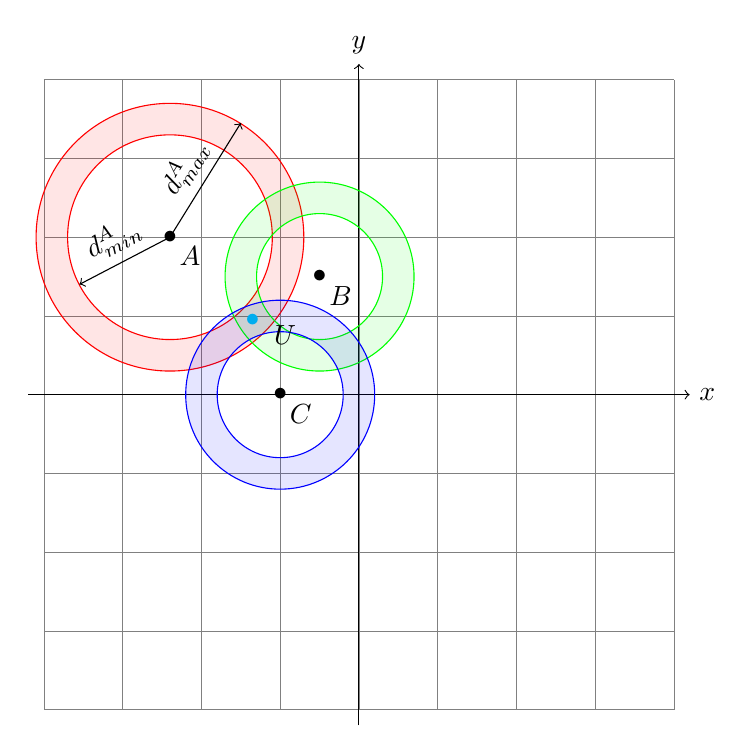
\begin{tikzpicture}
            \draw[very thin,color=gray] (-4,-4) grid (4,4);
            \draw[->] (-4.2,0) -- (4.2,0) node[right] {$x$};
            \draw[->] (0,-4.2) -- (0,4.2) node[above] {$y$};
    
            \draw[color=red] (-2.4,2) circle (1.5+0.2);
            \draw[color=red] (-2.4,2) circle (1.5-0.2);
            \fill [red,even odd rule,opacity=0.1] (-2.4,2) circle[radius=1.5+0.2] circle[radius=1.5-0.2];
            \draw[->](-2.4,2) -- (-1.5,3.45) node[midway,above,sloped] {$d^A_{max}$};
            \draw[->](-2.4,2) -- (-3.55,1.4) node[midway,above,sloped] {$d^A_{min}$};
            \draw (-2.4,2) node {$\bullet$};
            \node[anchor=north west] at (-2.4,2) {$A$};
        
            \draw[color=green] (-0.5,1.5) circle (1+0.2);
            \draw[color=green] (-0.5,1.5) circle (1-0.2);
            \fill [green,even odd rule,opacity=0.1] (-0.5,1.5) circle[radius=1+0.2] circle[radius=1-0.2];
            \draw (-0.5,1.5) node {$\bullet$};
            \node[anchor=north west] at (-0.5,1.5) {$B$};
        
            \draw[color=blue] (-1,0) circle (1+0.2); %2-2sqrt(3)
            \draw[color=blue] (-1,0) circle (1-0.2);
            \fill [blue,even odd rule,opacity=0.1] (-1,0) circle[radius=1+0.2] circle[radius=1-0.2];
            \draw (-1,0) node {$\bullet$};
            \node[anchor=north west] at (-1,0) {$C$};
            
            \draw (-1.35,0.95) [cyan] node {$\bullet$};
            \node[anchor=north west] at (-1.2,1) {$U$};
        \end{tikzpicture}
    }
    %\includegraphics{}
    \caption{}
    \label{fig:annulus}
\end{figure}
One important drawback is the low number of measurements exploited. Clearly, a higher number of samples implies a lower influence of the noise on the final estimation.
\clearpage

\section{Min Max 151}
  \begin{center}
  \textbf{Assume to know:}
  \begin{itemize}
    \centering
    \item $A$
    \item $\alpha$
  \end{itemize}
  \end{center}
Consider the previous framework. As usual one can deduce the distance of the unknown node, by reverting the propagation model as done in the previous section. Then we can obtain a number of circumferences, one for each anchor node, that represent the possible locations of the unknown node. In this algorithm however you need to consider not circles but squares. The case with three anchor node can be reviewed in \cite{inproceedings}, here it is presented a logical generalization of that method with multiple nodes. More precisely, each anchor node $i$ with estimated distance $d_i$ from $n_u$ is associated to a square centered in $(x_i,y_i)$ with side equal to $2d_i$. At this point, one has a set of overlapping squares, and can easily find the intersection of all those squares,  which results in a rectangles of vertices $(x_{min},x_{max},y_{min},y_{max})$ with the following equations:
\begin{equation}
    x_{min}=\max(x_1-d_1,...,x_n-d_n)
\end{equation}
\begin{equation}
    x_{max}=\min(x_1+d_1,...,x_n+d_n)
\end{equation}
\begin{equation}
    y_{min}=\max(y_1-d_1,...,y_n-d_n)
\end{equation}
\begin{equation}
    y_{max}=\min(y_1+d_1,...,y_n+d_n)
\end{equation}
The final location will be estimated as the center of this rectangle, as follows:
\begin{equation}
    x_t=\frac{x_{min}+x_{max}}{2}
\end{equation}
\begin{equation}
    y_t=\frac{y_{min}+y_{max}}{2}
\end{equation}
The gray area in \ref{fig:mmax} shows the intersection of all the squares. The estimated point will be obtained as the center of this rectangle.
\begin{figure}
    \centering
    \scalebox{1.3}{
        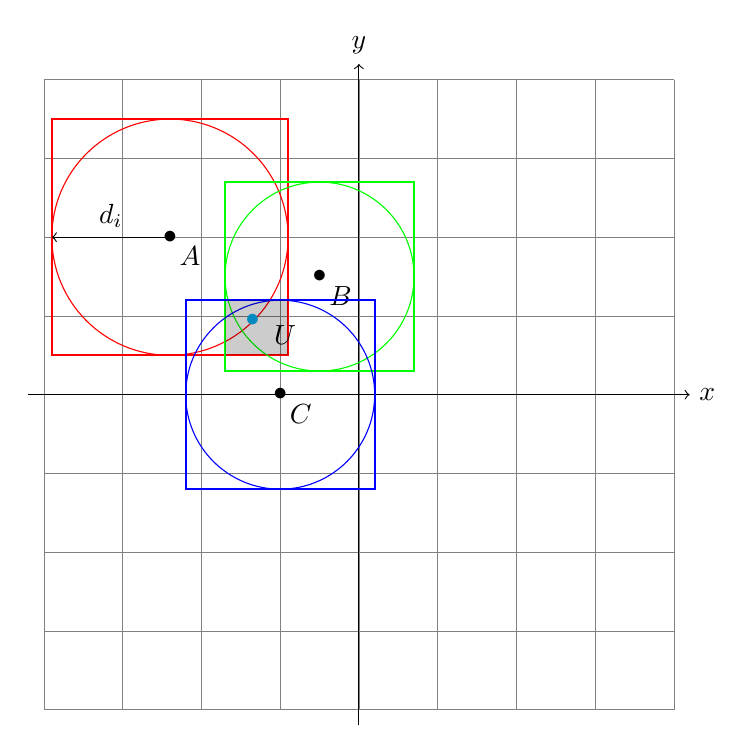
\begin{tikzpicture}
            \draw[very thin,color=gray] (-4,-4) grid (4,4);
            \draw[->] (-4.2,0) -- (4.2,0) node[right] {$x$};
            \draw[->] (0,-4.2) -- (0,4.2) node[above] {$y$};
    
            \draw[color=red] (-2.4,2) circle (1.5);
            \draw[red, thick] (-3.9,0.5) rectangle (-0.9,3.5);
            \draw[->](-2.4,2) -- (-3.9,2) node[midway,above,sloped] {$d_i$};
            \draw (-2.4,2) node {$\bullet$};
            \node[anchor=north west] at (-2.4,2) {$A$};
        
            \draw[color=green] (-0.5,1.5) circle (1.2);
            \draw[green, thick] (-1.7,0.3) rectangle (0.7,2.7);
            \draw (-0.5,1.5) node {$\bullet$};
            \node[anchor=north west] at (-0.5,1.5) {$B$};
        
            \draw[color=blue] (-1,0) circle (1.2); %2-2sqrt(3)
            \draw[blue, thick] (-2.2,-1.2) rectangle (0.2,1.2);
            \draw (-1,0) node {$\bullet$};
            \node[anchor=north west] at (-1,0) {$C$};
            
            \draw (-1.35,0.95) [cyan] node {$\bullet$};
            \node[anchor=north west] at (-1.2,1) {$U$};
            
            \fill [opacity=0.2] (-0.9,1.2) rectangle (-1.7,0.5);
        \end{tikzpicture}
    }
    %\includegraphics{}
    \caption{}
    \label{fig:mmax}
\end{figure}
does it always converge? $x_max$ is always greater than $x_min$?
\clearpage

\section{Linear estimation 881}
  \begin{center}
  \textbf{Assume to know:}
  \begin{itemize}
    \centering
    \item $A$
    \item $\alpha$
    \item $\xi_i,\forall i$
  \end{itemize}
  \end{center}
In \cite{rzk} you can find this version but using a slighty different model.
Consider the model ?? below reported
\begin{equation}
    \nu_i=-\beta\ln(d_i)+\xi_i
\end{equation}
After some time, for each anchor node we will have a list of measurements, drawn from the random variable 
\begin{equation}
N_i=-\beta\ln(d_i)+\xi_i.
\end{equation}
Cite ross also here, only for $\mathcal{N}+a$, and remind $xi_i\sim\mathcal{N}(0,\sigma^2_i)$. To give an idea, each anchor node outputs data as a gaussian distribution shifted by the mean, so for the anchor node we have samples extracted from $\mathcal{N}(-\beta\ln(d_i), \sigma_i^2)$. Note that $\sigma_i$ is not necessarily contant, for all $i$.

Rewrite the ?? as follows 
\begin{equation}
    \nu_i=-\ln\big(d_i^{2\frac{\beta}{2}}\big)+\xi_i
\end{equation}
By exponentiating both members of ??(previous) we have 
\begin{equation}
    e^{\nu_i}=e^{-\ln\big(d_i^{2\frac{\beta}{2}}\big)+\xi_i}
\end{equation}
\begin{equation}
    \bigg(e^{\nu_i}\bigg)^{-1}=\bigg(e^{-\ln\big(d_i^{2\frac{\beta}{2}}\big)+\xi_i}\bigg)^{-1}
\end{equation}
\begin{equation}
    e^{-\nu_i}=e^{\ln\big(d_i^{2\frac{\beta}{2}}\big)-\xi_i}
\end{equation}
\begin{equation}
    e^{-\nu_i}=d_i^{2\frac{\beta}{2}}e^{-\xi_i}
\end{equation}
\begin{equation}
    \bigg(e^{-\nu_i}\bigg)^{\frac{2}{\beta}}=\bigg(d_i^{2\frac{\beta}{2}}e^{-\xi_i}\bigg)^{\frac{2}{\beta}}
\end{equation}
\begin{equation}
    e^{-\frac{2}{\beta}\nu_i}=d_i^2e^{-\frac{2}{\beta}\xi_i}
\end{equation}
Remind that $\xi_i\sim \mathcal{N}(0,\sigma^2_i)$ is a zero-mean gaussian distribution. The exponentiation of a gaussian distribution is \cite{Beran2011} a log-normal distribution. In other words, given $X\sim \mathcal{N}(\mu,\sigma^2)$, then $Y=e^X\sim \text{Lognormal}(\mu,\sigma^2)$ with
\begin{equation}
    E[Y]=E\big[e^X\big]=e^{\mu+\frac{\sigma^2}{2}}
\end{equation}
\begin{equation}
    Var[Y]=Var\big[e^X\big]=(e^{\sigma^2}-1)e^{2\mu+\sigma^2}
\end{equation}
From \cite{alma9926534668905776}, it is clear that if $a\in \mathbb{R}$ and $X\sim \mathcal{N}(\mu,\sigma^2)$ then
\begin{equation}
aX\sim \mathcal{N}(a\mu,a^2\sigma^2)    
\end{equation}
so in this case, 
\begin{equation}
    -\frac{2}{\beta}\xi_i\sim \mathcal{N}\bigg(0,\frac{4}{\beta^2}\sigma^2_i\bigg)
\end{equation}
From equations ?? and ?? (previous equation)
\begin{align}
    &E\bigg[e^{-\frac{2}{\beta}\nu_i}\bigg]\\
    &=E\bigg[d_i^2e^{-\frac{2}{\beta}\xi_i}\bigg]\\
    &=d_i^2E\bigg[e^{-\frac{2}{\beta}\xi_i}\bigg]\\ &=d_i^2e^{\frac{2}{\beta^2}\sigma^2_i}
\end{align}
\begin{align}
    &Var\bigg[e^{-\frac{2}{\beta}\nu_i}\bigg]\\
    &=Var\bigg[d_i^2e^{-\frac{2}{\beta}\xi_i}\bigg]\\
    &=d_i^4Var\bigg[e^{-\frac{2}{\beta}\xi_i}\bigg]\\
    &=d_i^4(e^{\frac{4}{\beta^2}\sigma_i^2}-1)e^{\frac{4}{\beta^2}\sigma^2_i}
\end{align}
As we can see from ??, $e^{-\frac{2}{\beta}\nu_i}$ is a biased estimate of $d_i^2$ since from ?? its mean is not $d_i^2$ as we wanted, however we can remove its bias by dividing it by $e^{\frac{2}{\beta^2}\sigma^2_i}$. Therefore, an unbiased estimate of $d_i^2$ is 
\begin{equation}
    \hat{d}_i^2=e^{-\frac{2}{\beta}\nu_i-\frac{2}{\beta^2}\sigma^2_i}
\end{equation}
We want to use the above estimator obtained from the measurements to build a linear models in $\mathbf{x}$. Since the estimator is now unbiased by writing 
\begin{equation}
    \hat{d}_i^2=(x-x_i)^2+(y-y_i)^2
\end{equation}
we can write
\begin{equation}
    (x-x_i)^2+(y-y_i)^2=e^{-\frac{2}{\beta}\nu_i-\frac{2}{\beta^2}\sigma^2_i}
\end{equation}
\begin{equation}
    -2x_ix-2y_iy+x^2+y^2+x_i^2+y_i^2=e^{-\frac{2}{\beta}\nu_i-\frac{2}{\beta^2}\sigma^2_i}
\end{equation}
\begin{equation}
    -2x_ix-2y_iy+x^2+y^2=e^{-\frac{2}{\beta}\nu_i-\frac{2}{\beta^2}\sigma^2_i}-x_i^2-y_i^2
\end{equation}
By setting the condition 
\begin{equation}
R^2=x^2+y^2    
\end{equation}
we can write it in matrix form
\begin{equation}
    \begin{bmatrix}
        -2x_1 & -2y_1 & 1\\
        \vdots&\vdots&\vdots\\
        -2x_n & -2y_n & 1
    \end{bmatrix}
    \begin{bmatrix}
        x\\
        y\\
        R^2
    \end{bmatrix} = 
    \begin{bmatrix}
       e^{-\frac{2}{\beta}\nu_1-\frac{2}{\beta^2}\sigma^2_1} & -x_1^2 & -y_1^2\\
        \vdots&\vdots&\vdots\\
        e^{-\frac{2}{\beta}\nu_n-\frac{2}{\beta^2}\sigma^2_n} & -x_n^2 & -y_n^2\\
    \end{bmatrix}
\end{equation}
with $$M=\begin{bmatrix}
        -2x_1 & -2y_1 & 1\\
        \vdots&\vdots&\vdots\\
        -2x_n & -2y_n & 1
    \end{bmatrix}$$
$$\theta^* =     \begin{bmatrix}
        x\\
        y\\
        R^2
    \end{bmatrix}$$
$$b=    \begin{bmatrix}
        e^{-\frac{2}{\beta}\nu_1-\frac{2}{\beta^2}\sigma^2_1} & -x_1^2 & -y_1^2\\
        \vdots&\vdots&\vdots\\
        e^{-\frac{2}{\beta}\nu_n-\frac{2}{\beta^2}\sigma^2_n} & -x_n^2 & -y_n^2\\
    \end{bmatrix}$$
Now since $\theta^*$ is unknown we would like to choose $\theta\approx\theta^*$ to have 
\begin{equation}
    M\theta-b\approx0
\end{equation}
One easy way is to seek the minimum of 
\begin{align}
    J&(\theta)=(M\theta - b)^T(M\theta - b)\\
    &=\theta^TM^TM\theta-2\theta^TM^Tb+b^Tb
\end{align}
We can fit this model with the Least Square Method, that for a linear model (which is the ours) has a known explicit solution \cite{10.5555/1557273} that can be easily verified. In fact since $J(\theta)$ is a quadratic function of $\theta$, then there is a unique minimum \cite{Ortega1987,rzk}. The LLS estimate corresponds to:
\begin{equation}
    \hat{\theta}=\arg \min_\theta J(\theta)
\end{equation}
which can be found setting to $0$ its derivative
    
\begin{align}
\begin{split}
&\frac{\partial J(\theta)}{\partial \theta}=0\\
    &2M^TM\hat{\theta}-2M^Tb=0\\
    &A^TA\hat{\theta}=A^Tb\\
    &\hat{\theta}=(M^TM)^{-1}M^Tb
\end{split}
\end{align}


The target position can be finally obtained as 
\begin{equation}
\begin{bmatrix}
    \hat{x}\\
    \hat{y}
\end{bmatrix}=
\begin{bmatrix}
    [\hat{\theta}]_1\\
    [\hat{\theta}]_2
\end{bmatrix}
\end{equation}
\clearpage


\section{Weighted linear estimation 270}
In section ?? we have seen how to use statistics to obtain an estimator of the distance for each anchor node to the unknown node, and then putting all this in a linear form, to deduce the location of the unknown node with a simple closed formula such as the Linear least squares. However we can still improve it by givin to each anchor node a weight, bound to the variance of the estimator $\hat{d}_i^2$ obtained from the anchor node $i$. A good idea would be to give more importance to the nodes that produces an estimator with low variance, and to give less importance to those node that produces estimators with high variance. To ease the computation we consider each anchor node to be indepentendet from each other. One way to do that is to introduce a symmetric covariance matrix, diagonal (because of the independence of anchor nodes). Since we want the weight assigned to each node to be inversely proportional to the variance we consider $W=(W')^{-1}$ \cite{rzk,899498y4hd}. It is important to note that this improvement does not regard the generation of the vector of estimators, rather the minimization of the cost function. Now we compute the variance of each estimator $\hat{d}_i^2$, from ??
\begin{align}
Var&\big[\hat{d_i^2}\big]=&& \text{comment example } x\\
&=Var\bigg[e^{-\frac{2}{\beta}\nu_i-\frac{2}{\beta^2}\sigma^2_i}\bigg]\\
&=\bigg(e^{-\frac{2}{\beta^2}\sigma^2_i}\bigg)^2Var\bigg[e^{-\frac{2}{\beta}\nu_i}\bigg]\\
&=\cancel{e^{-\frac{4}{\beta^2}\sigma^2_i}}d_i^4\bigg(e^{\frac{4}{\beta^2}\sigma_i^2}-1\bigg)\cancel{e^{\frac{4}{\beta^2}\sigma^2}}\\
&=d_i^4\bigg(e^{\frac{4}{\beta^2}\sigma_i^2}-1\bigg)\\
&\approx \big(\hat{d_i}^2\big)^2\bigg(e^{\frac{4}{\beta^2}\sigma_i^2}-1\bigg)\\
&=\bigg(e^{-\frac{2}{\beta}\nu_i-\frac{2}{\beta^2}\sigma^2_i}\bigg)^2\bigg(e^{\frac{4}{\beta^2}\sigma_i^2}-1\bigg)\\
&=e^{-\frac{4}{\beta}\nu_i-\frac{4}{\beta^2}\sigma^2_i}\bigg(e^{\frac{4}{\beta^2}\sigma^2_i}-1\bigg)\\
&=e^{-\frac{4}{\beta}\nu_i}\bigg(1-e^{-\frac{4}{\beta^2}\sigma^2_i}\bigg)\\
&=\frac{1-e^{-\frac{4}{\beta^2}\sigma^2_i}}{e^{\frac{4}{\beta}\nu_i}}
\end{align}
Now we get to the weighting matrix
\begin{align}
    &\mathbf{W}=\text{diag}\big((\sigma^2_{d_1})^{-1},...,(\sigma^2_{d_n})^{-1}\big)\\
    &=\text{diag}\bigg(\frac{e^{\frac{4}{\beta}\nu_1}}{1-e^{-\frac{4}{\beta^2}\sigma^2_1}},...,\frac{e^{\frac{4}{\beta}\nu_n}}{1-e^{-\frac{4}{\beta^2}\sigma^2_n}}\bigg)
\end{align}
The improved cost function \cite{rzk} takes the following form 
\begin{align}
    J&(\theta)=(M\theta - b)^TW(M\theta - b)\\
    &=\theta^TM^TWM\theta-2\theta^TM^TWb+b^TWb
\end{align}
that can be minimized with the usual LLS
\begin{align}
    \hat{\theta}=(M^TWM)^{-1}M^TWb
\end{align}
The precision of this estimation can be further improved by imposing the constraint ?? ($\hat{\theta}_3=\hat{R}^2$) on the minimization. This condition is ignored if we use LLS, but it can be successfully employed with the method of Lagrange multipliers \cite{1275684,Lopez1994, pasa}.


\clearpage

\section{Quadratic linearization 510}
  \begin{center}
  \textbf{Assume to know:}
  \begin{itemize}
    \centering
    \item $A$
    \item $\alpha$
  \end{itemize}
  \end{center}
From the canonical model extract $d_i$ as follows
\begin{equation*}
    10^{RSSI_{i}}=10^{A-\alpha\log_{10}(d_i)}
\end{equation*}
\begin{equation*}
    10^{RSSI_{i}-A}=10^{-\alpha\log_{10}(d_i)}
\end{equation*}
\begin{equation*}
     10^{RSSI_{i}-A}=d_i^{-\alpha}
\end{equation*}
\begin{equation}
    d_i=10^{\frac{A-RSSI_{i}}{\alpha}}
\end{equation}
so that we have the following set of equations
\begin{align}
\begin{split} 
(x_1-x)^2+(y_1-y)^2&=d_1^2 \\ 
(x_2-x)^2+(y_2-y)^2&=d_2^2 \\ 
&\;\;\vdots\\
(x_n-x)^2+(y_n-y)^2&=d_n^2 \\
\end{split}
\end{align}
Consider 
\begin{align}
\frac{1}{n}&\sum_{i=1}^nd_i^2=\\
&=\frac{1}{n}\sum_{i=1}^n\big[(x_i-x)^2+(y_i-y)^2\big]\\
&=\frac{1}{n}\sum_{i=1}^n(x_i-x)^2+\frac{1}{n}\sum_{i=1}^n(y_i-y)^2\\
&=\frac{1}{n}\sum_{i=1}^n[x_i^2-2x_ix+x^2] + \frac{1}{n}\sum_{i=1}^n[y_i^2-2y_iy+y^2]\\
&=\frac{1}{n}\sum_{i=1}^n[x_i^2]-2x\frac{1}{n}\sum_{i=1}^n[x_i]+ x^2 + \frac{1}{n}\sum_{i=1}^n[y_i^2]-2y\frac{1}{n}\sum_{i=1}^n[y_i]+ y^2
\end{align}
Frone one of the ?? it follows
\begin{equation}
x_i^2+x^2-2x_ix+y_i^2+y^2-2y_iy=d_i^2      
\end{equation}
\begin{equation}
-x_i^2-x^2+2x_ix-y_i^2-y^2+2y_iy=-d_i^2      
\end{equation}
Now by adding ?? to ?? previous you have 
\begin{equation}
\begin{split}
    \bigg(-x_i^2  + \frac{1}{n}\sum_{i=1}^n[x_i^2]\bigg)+
    \bigg(-y_i^2+ \frac{1}{n}\sum_{i=1}^n[y_i^2]\bigg)+\\
    +\bigg(2x_ix-2x\frac{1}{n}\sum_{i=1}^n[x_i]\bigg)+
    \bigg(2y_iy -2y\frac{1}{n}\sum_{i=1}^n[y_i]\bigg)
    =\frac{1}{n}&\sum_{i=1}^n[d_i^2]-d_i^2
\end{split}    
\end{equation}
and by rearranging the equation
\begin{equation}
\begin{split}
    +2x\bigg(x_i-\frac{1}{n}\sum_{i=1}^n[x_i]\bigg)+
    2y\bigg(y_i -\frac{1}{n}\sum_{i=1}^n[y_i]\bigg)\\
    \bigg(-x_i^2  + \frac{1}{n}\sum_{i=1}^n[x_i^2]\bigg)+
    \bigg(-y_i^2+ \frac{1}{n}\sum_{i=1}^n[y_i^2]\bigg)
    =\frac{1}{n}&\sum_{i=1}^n[d_i^2]-d_i^2
\end{split}    
\end{equation}
then the previous set of equations ?? becomes
\begin{align}
\begin{split} 
    \bigg(x_1-\frac{1}{n}&\sum_{i=1}^nx_i\bigg)x+\bigg(y_1-\frac{1}{n}\sum_{i=1}^ny_i\bigg)y\\
    &=\frac{1}{2}\bigg[\bigg(x_1^2-\frac{1}{n}\sum_{i=1}^nx^2_i\bigg)+\bigg(y_1^2-\frac{1}{n}\sum_{i=1}^ny^2_i\bigg)-\bigg(d_1^2-\frac{1}{n}\sum_{i=1}^nd_i^2\bigg)\bigg]\\
&\;\;\vdots\\
    \bigg(x_n-\frac{1}{n}&\sum_{i=1}^nx_i\bigg)x+\bigg(y_n-\frac{1}{n}\sum_{i=1}^ny_i\bigg)y\\
    &=\frac{1}{2}\bigg[\bigg(x_n^2-\frac{1}{n}\sum_{i=1}^nx^2_i\bigg)+\bigg(y_n^2-\frac{1}{n}\sum_{i=1}^ny^2_i\bigg)-\bigg(d_n^2-\frac{1}{n}\sum_{i=1}^nd_i^2\bigg)\bigg]
\end{split}
\end{align}
So can write the above set of equations in matricial form $\mathbf{Mx}=\mathbf{b}$ by setting
$$
\mathbf{M}=\begin{bmatrix}
    x_1-\frac{1}{n}\sum_{i=1}^nx_i&y_1-\frac{1}{n}\sum_{i=1}^ny_i\\
    \vdots&\vdots\\
    x_n-\frac{1}{n}\sum_{i=1}^nx_i&y_n-\frac{1}{n}\sum_{i=1}^ny_i
\end{bmatrix}
$$
$$
\mathbf{x}=\begin{bmatrix}
    x\\
    y
\end{bmatrix}
$$
$$\mathbf{b}=\frac{1}{2}
\begin{bmatrix}
\bigg(x_1^2-\frac{1}{n}\sum_{i=1}^nx^2_i\bigg)+\bigg(y_i^2-\frac{1}{n}\sum_{i=1}^ny^2_i\bigg)-\bigg(d_i^2-\frac{1}{n}\sum_{i=1}^nd_i^2\bigg)\\
\vdots\\
\bigg(x_n^2-\frac{1}{n}\sum_{i=1}^nx^2_i\bigg)+\bigg(y_n^2-\frac{1}{n}\sum_{i=1}^ny^2_i\bigg)-\bigg(d_n^2-\frac{1}{n}\sum_{i=1}^nd_i^2\bigg)
\end{bmatrix}
$$
then the solution can be computed with the usual Linear Least Square procedure obtaining
\begin{equation}
    \mathbf{x}=(\mathbf{M^TM})^{-1}\mathbf{M^Tb}
\end{equation}
Also valid for non RSSI based localization
\clearpage


\section{Lines intersection 858}
Let's start from a geometrical analysis. Given two intersecting circles at center $x_{1},y_{1}$ and $x_{2},y_{2}$ respectively and with radius $r_1$ and $r_2$ respectively, the line that passes by the two points of intersection has the following equation
\begin{equation}
    (x_2-x_1)x+(y_2-y_1)y=\frac{1}{2}\big[(x_2^2+y_2^2)-(x_1^2+y_1^2)-(r_2^2-r_1^2)\big]
\end{equation}
from subtracting one equation of the circle to the other. Now a question arise, given the noise effect on the measurements, what happens if the two circles are not intersecting? Is the formula still valid? Yes. Why?... 

The formula can be obtained by deriving $m$ and $q$. The parameter $m$ in the perpendicular to line passing between the two centers.

Given $n$ measurements (so $n$ circles), only $n-1$ are needed to have an independent system of equations. For example, for the trilateration method, (thus with three circles), it is needed to have only 2 lines, for example the line passing between the first and the second circle, and the line passing between the first and the third one. (optimization! given instead using only the first circle use the previous one: (1,2), (1,3) use (1,2), (2,3)).
Therefore, given $n$ points we have a set of $n-1$ equations like the above ??, that can be written in matricial form $\mathbf{Mx}=\mathbf{b}$ with
$$\mathbf{M}=\begin{bmatrix}
x_2-x_1&y_2-y_1\\
x_3-x_1&y_3-y_1\\
\vdots&\vdots\\
x_n-x_1&y_n-y_1
\end{bmatrix}$$
$$\mathbf{x}=\begin{bmatrix}
x\\
y
\end{bmatrix}$$
$$\mathbf{b}=\begin{bmatrix}
(x^2_2+y^2_2)-(x_1^2+y^2_1)-(d_2^2-d_1^2)\\
(x^2_3+y^2_3)-(x_1^2+y^2_1)-(d_3^2-d_1^2)\\
\vdots\\
(x^2_n+y^2_n)-(x_1^2+y^2_1)-(d_n^2-d_1^2)\\
\end{bmatrix}$$
The solution is obtained as an approximated intersection of all these lines with the LLS.

Given the high influence in this formula of the first anchor node (present in all equations), one can try an optimization by rearranging the above formula in a way that it relays more evenly to the all nodes as follows
$$\mathbf{M}=\begin{bmatrix}
x_2-x_1&y_2-y_1\\
x_3-x_2&y_3-y_2\\
\vdots&\vdots\\
x_n-x_{n-1}&y_n-y_{n-1}
\end{bmatrix}$$
$$\mathbf{x}=\begin{bmatrix}
x\\
y
\end{bmatrix}$$
$$\mathbf{b}=\begin{bmatrix}
(x^2_2+y^2_2)-(x_1^2+y^2_1)-(d_2^2-d_1^2)\\
(x^2_3+y^2_3)-(x_2^2+y^2_2)-(d_3^2-d_2^2)\\
\vdots\\
(x^2_n+y^2_n)-(x_{n-1}^2+y^2_{n-1})-(d_n^2-d_{n-1}^2)\\
\end{bmatrix}$$
Highly resistant to noise. Always gives a result. Fast.
\clearpage


\section{Multilateration 435}
(We can also set many different $\alpha_i$ one for each node deduced with previous chapter)
Disadvantage, need a starting point quite close to the actual location, maybe estimated with some of the above methods, otherwise it diverges.
If you assume to know $A$ then good results with GN method...\\
This algorithm is the generalization of the trilateration method, and is known as multilateration. 
This method can provide two main benefits over the classic trilateration:
\begin{itemize}
    \item Always exists a solution (the algorithm may not be able to find it though)
    \item The result is made on more observation than the trilateration
\end{itemize}
The first point can be explained as follows:
We start by measuring the rssi value in each position.This measurement can be fitted to the model of $RSSI$ propagation. Assuming that the exact distribution follows 
\begin{equation}
rssi(x,y)=A^*-10\alpha^*\log_{10}\big(\sqrt{(x_t^*-x)^2+(y_t^*-y)^2}\big)    
\end{equation}
with $A^*,\alpha^*,x^*_t,y^*_t$ unknown, we can write a performance index $J$
\begin{equation}
    J(A,n,x_t,y_t)=\sum_{i=1}^n\bigg(rssi_i-A+10\alpha\log_{10}\big(\sqrt{(x_i-x_t)^2+(y_i-y_t)^2}\big)\bigg)
\end{equation}
and then choosing 
\begin{equation}
\Bar{x_t}, \Bar{y_t}=\arg \min_{A,\alpha,x_t,y_t}J(A,\alpha,x_t,y_t)
\end{equation}
\clearpage


\section{Maximum Likelihood method 486}
When the error follows a zero mean gaussian distribution, this method is a weighted version of the Nonlinear Multilateration method. 
\begin{equation}
    \beta=\frac{\alpha}{\ln(10)}
\end{equation}
Each anchor $i$ has a distribution like $\mathcal{N}(-\beta\ln(d_i),\sigma^2_i)$
A look more closely related to the probability point of view is
\begin{equation}
    \pi(\nu_i)=\frac{1}{\sqrt{2\pi\sigma^2_{\nu_i}}}e^{-\frac{1}{2}\frac{(\nu_i+\alpha\ln(d_i))^2}{\sigma^2_{\nu_i}}}
\end{equation}
$\mathbf{\Sigma}$ is diagonal for uncorrelated (remember independent implies uncorrelated, but not the reverse) variables
$$\mathbf{f}(\mathbf{x})=-\beta\begin{bmatrix}
\ln(\sqrt{(x-x_1)^2+(y-y_1)^2})\\
\vdots\\
\ln(\sqrt{(x-x_n)^2+(y-y_n)^2})
\end{bmatrix}$$
For $n$ indepentent and (identically? mean is the value read which changes) distributed, the joint probabilty distribution is the product
\begin{equation}
    \pi(\mathbf{RSS})=\frac{1}{(2\pi)^{\frac{n}{2}}\Pi_{i=1}^n\sigma_{\nu_i}}e^{-\frac{1}{2}\sum_{i=1}^n\frac{(\nu_i+\alpha\ln(d_i))^2}{\sigma^2_{\nu_i}}}
\end{equation}
\begin{equation}
    \pi(\mathbf{r}_{RSS})=\frac{1}{(2\pi)^{\frac{n}{2}}|\mathbf{\Sigma}|^{\frac{1}{2}}}e^{-\frac{1}{2}\big(\mathbf{r}_{RSS}-\mathbf{f}(\mathbf{x})\big)\mathbf{\Sigma}^{-1}\big(\mathbf{r}_{RSS}-\mathbf{f}(\mathbf{x})\big)}
\end{equation}
For the Maximum Likelihood method we need to find the minimum of ??. To facilitate it we consider the log. The first part is independent of x, so we need only to maxmize the second part. We can now remove the logarithm because it is a monotonic increasing function, then we oibtain the previous forumula to be minimized. As you can see when $\mathbf{\Sigma}=diag{(\sigma_1,...)}$. The solution can be found with Newton raphson, GN...

\clearpage

From \cite{KAUR201982} and also each bibliography
\section{Centroid algorithm 677}
\begin{algorithm}[H]
\SetAlgoLined
\KwResult{Estimated position of the unknown node}
 Each node $i$ broadcasts its position $(x_i,y_i)$ to every other node\;
 Define threshold\;
 Each anchor node retain the information of the nodes that are above the threshold\;
 The unknown node computes its position as:
 \begin{equation}
     x_u=\frac{\sum_{i=1}^mx_i}{m},\quad y_u=\frac{\sum_{i=1}^my_i}{m}
 \end{equation}
 which is the mean of the position of the retained nodes.
 \caption{Centroid algorithm}
\end{algorithm}
\noindent\\From \cite{878533} the threshold can be calculated in two ways. The first method consists of a simple selection based on the rssi level, that is, every nearest node (whose level is above the rssi threshold) is kept. The second method employs a more sofisticated approach. Every node broadcasts multiple packets in the network, then each node replies with one packet per packet received. Therefore we can draw a list for every node $i$ as follows 
\begin{equation}
    g_i = \frac{\text{n. of packets sent to node $i$}}{\text{n. of packets received from node $i$}}
\end{equation}
Since the quality/quantity of packets degrades with the distance, closer node will have a higher grade, while farther nodes will have a lower one. Then only the packets with a grade greather or equal to a certain threshold (e.g. $0.9$) will be considered. This is a quite simple algorithm, since it assumes that the nodes with known position are positioned in a regular grid. It presents however low accuracy, and also it may be difficult to determine threshold value. The main advantage however is the simultaneous localization of multiple unknown nodes. Below a possible arrangement (known nodes in grid, unknoen node random, with a circle around to set the threshold). There exists some improvements of the previous algorithm, for example the Weighted Centroid Algorithm. The new metric Just use $w_{u,i}=\frac{1}{h_{u,i}}$ h is hop count, then centroid is weighted, not simple average.
(new algorithm here)
\clearpage

\section{DV-Hop Algorithm 422}
The DV-Hop algorithm was first published by in \cite{965964}.\\
\begin{algorithm}[H]
\SetAlgoLined
\KwResult{Estimated position of the unknown node}
Each node has the minimum hop count from itself to each node\;
Each node compute average 
\begin{equation}
    AvgHopDistance_i=\frac{\sum_{i=1,i\neq j}^m\sqrt{(x_j-x_i)^2+(y_j-y_i)^2}}{\sum_{i=1,i\neq j}^mh_{j,i}}
\end{equation}\\
Each unknown node $u$ computes the approximate distance from anchor node i using 
\begin{equation}
    d_{u,i}=AvgHopDistance_i \cdot h_{u,i}
\end{equation}
 \caption{DV-Hop algorithm}
\end{algorithm}
\noindent\\
The algorithm begins with a broadcast of all nodes with a packet, that contains informations about its position and the hop count, which starts from zero and it is incremented by at each node it passes through. Each node upgrade its metrics accordingly. After some time necessary to reach a stable point where no information update happen, we have a situation where every node has the minimum hop count from itself to each node and the positions of each node in a table like... (table here). (picture of some nodes, show many paths, show the one with less hop counts) For example, node A has 2 path to reach node B, but the path abababa has hop count = 3...
As soon as the data is available each unknown node can compute its approximated distance from each node $i $ as in line $3$ of the Algo ??. Therefore each unknown node $u$ is able to derive the following equations
\begin{align}
\begin{split} 
(x_1-x_u)^2+(y_1-y_u)^2&=d_{u,1}^2 \\ 
(x_2-x_u)^2+(y_2-y_u)^2&=d_{u,2}^2 \\ 
&\;\;\vdots\\
(x_n-x_u)^2+(y_n-y_u)^2&=d_{u,n}^2 \\
\end{split}
\end{align} 
where $d_{u,i}$ is the distance (in meters) from node $u$ to node $i$.
By subtracting the $n$-th equation to all the others, those can be transformed to
\begin{align}
\begin{split} 
x_1^2-x_m^2+y_1^2-d_{u,1}^2-d_{u,n}^2&=2x_u(x_1-x_n)+2y_u(y_1-y_u)\\ 
x_2^2-x_m^2+y_2^2-d_{u,2}^2-d_{u,n}^2&=2x_u(x_2-x_n)+2y_u(y_2-y_u)\\
&\;\;\vdots\\
x_2^2-x_m^2+y_2^2-d_{u,2}^2-d_{u,n}^2&=2x_u(x_{n-1}-x_n)+2y_u(y_2-y_u)
\end{split}
\end{align}
Can be written in matrix form $AX_u=B$
where 
\begin{equation}
    A=2\begin{bmatrix}
    x_1-x_m & y_1-y_m\\
    x_2-x_m & y_2-y_m\\
    \vdots & \vdots\\
    x_{m-1}-x_m & y_{m-1}-y_m
    \end{bmatrix}
\end{equation}
\begin{equation}
    X_u=\begin{bmatrix}
    x_u\\
    y_u
    \end{bmatrix}
\end{equation}
\begin{equation}
    B=\begin{bmatrix}
        x_{1}^2-x_m^2+y_{1}^2-y_m^2-d_{u,1}^2-d^2_{u,m}\\
        x_{2}^2-x_m^2+y_{2}^2-y_m^2-d_{u,2}^2-d^2_{u,m}\\
        \vdots\\
        x_{m-1}^2-x_m^2+y_{m-1}^2-y_m^2-d_{u,n-1}^2-d^2_{u,m}
    \end{bmatrix}
\end{equation}
The result can be computed with the closed formula of the LLS
\begin{equation}
    X_u=(A^TA)^{-1}A^TB
\end{equation}
\clearpage


\section{Fingerprinting 437}
from \cite{YIU2017235} 1-NN compares how each anchor node sees all the other nodes to how the unknown node reads the rssi of all the anchor nodes. Then the estimated location would be the anchor node closest to the unknown node. kNN takes the mean of the first k\\\\\\
Fingerprinting is a quite general technique, that can be used for many scenarios. Its main drawback is the offline training phase, that need to be done before the localization takes place, therefore its use is mostly reserved for example for the location of devices in a known area, that can be for example factories, shpping center, where the nodes have all the time to acquire a precise and accurate representation of the normal environment. As soon as this phase is done, it can start the localization phase. The main principle underlying this method is the analysis of the similarity of signals intensity observed by the unknown node w.r.t. the other nodes. The algorithm employed by this method is known as K-NN or K nearest neighbours \cite{10.5555/1162264}. Here it is presented the version working with $1-NN$, 
In the learining (offline) phase, every node build an internal database with records of every node along with the received signal strength as in the the following table (table). As soon as the localization phase starts, (centralized algorithm?) the following formula is used
\begin{equation}
    \hat{i}=\arg \min_{\mathbf{x_h}}\bigg\{\sum_{k=1}^n(r_i(k)-r_{n+1(k)})^2\bigg\}
\end{equation}
metti meglio, descrivi $(...)^2$ come cifra di merito,
dunque questo algoritmo seleziona il nodo $i$ tale per cui la somma delle differenze di come il nodo $i$ vede tutti i nodi diversi da $i$ sia minore, ovvero, ideally, that, according to the signal intensity read, it should be closest to the unknown node. The estimated position is that node. Clearly this is a quite raw estimation, since can take only one out of the $n$ known positions, but in can be efficiently improved for higher values of $k$. In those cases, the selected nodes are $k$, and the final estimate is computed as the mean of the position of those $k$ nodes, as the name says, the $k$ nearest neighbours.  


\chapter{Conclusioni (1 pag)}
Advantages of drone.... however the employement of anchor nodes remains a good option (deduce itself parameters...)








\clearpage
\printbibliography[
heading=bibintoc,
title={Whole bibliography}
]
%Prints the entire bibliography with the title "Whole bibliography"

%\clearpage

%Filters bibliography
%\printbibliography[heading=subbibintoc,type=article,title={Articles only}]
%\printbibliography[type=book,title={Books only}]
%\printbibliography[keyword={physics},title={Physics-related only}]
%\printbibliography[keyword={latex},title={\LaTeX-related only}]

\end{document}
